\section{Adhoc-Netzwerke}\label{s:AdhocNetzwerke}

Adhoc-Netze sind in sich geschlossene Netzwerke, organisieren sich selbst und haben keine bestimmte Hierarchie. Sie bauen sich nur für die Dauer einer Datenübertragung auf, besitzen keine festgelegte Kommunikationsstruktur und verwalten und organiseren sich selbst. 

Adhoc-Netze sind leistungsfähige und zählen als so genanntes 'Self Organized Network' (SON), welche gute Lastverteilung betreiben und ohne zentrales Management auskommen. Die Endgeräte übernehmen in diesem Fall das Routing und speichern die Routingtabellen selbst ab. Geräte, die sich dem Netzwerk anschließen, werden dynamisch in das Netz eingefügt. Bei Netzwerken nach IEEE 802.11 (WLANs) und IEEE 802.15 (WPANs - hier im Speziellen IEEE 802.15.1 - Bluetooth) werden alle Geräte selbstständig erkannt und werden dem Netz hinzugefügt. Sie sind fortan Bestandteil des Gesamtnetzes. 

Bei Adhoc-Netzen mit vielen Geräten (das kann z.B. ein Sensornetz sein) wird zumeist eine Multihop-Verbindung bevorzugt. Das bedeutet, dass die Daten von einem Netzknoten, z.B. einem Sensor oder Rechner, zu dem nächsten Netzknoten weitergeleitet werden, bis es sein Ziel erreicht hat. Fällt ein Knoten aus, wird wenn möglich ein anderer Weg für die Übertragung genutzt, um Ausfälle zu vermeiden.

Ad-hoc-Netzwerke bestehen virtuell für einen begrenzten Zeitrahmen. Ad-hoc bedeutet etwa "für den Augenblick gemacht". Sie werden in WLANs, WPANs, in Sensornetzen (WPANs mit geringer Datenrate - siehe IEEE 802.15.4) und in Funknetzen von Rettungsdiensten, Polizei und Militär benutzt \cite{ws:lipinski}.

\subsection{MANETs}\label{ss:MANETs}

MANET bezeichnet die Abkürzung für den Begriff ‚Mobile Ad-hoc Network‘. Jochen Schiller beschreibt in seiner Literatur „Mobile Communications“ den Begriff des MANETs wie folgt: „Ad-hoc-Netze kommen ohne jegliche Infrastruktur aus, insbesondere ohne eine ausgezeichnete Basisstation, welche den Medienzugriff zentral steuert. Diese Netzvariante erlaubt die spontane, nicht vorab geplante Kommunikation zwischen mobilen Endgeräten, wobei einige oder alle Endgeräte auch Daten von anderen Endgeräten weiterleiten können.“

\begin{figure}[H] 
	\centering
	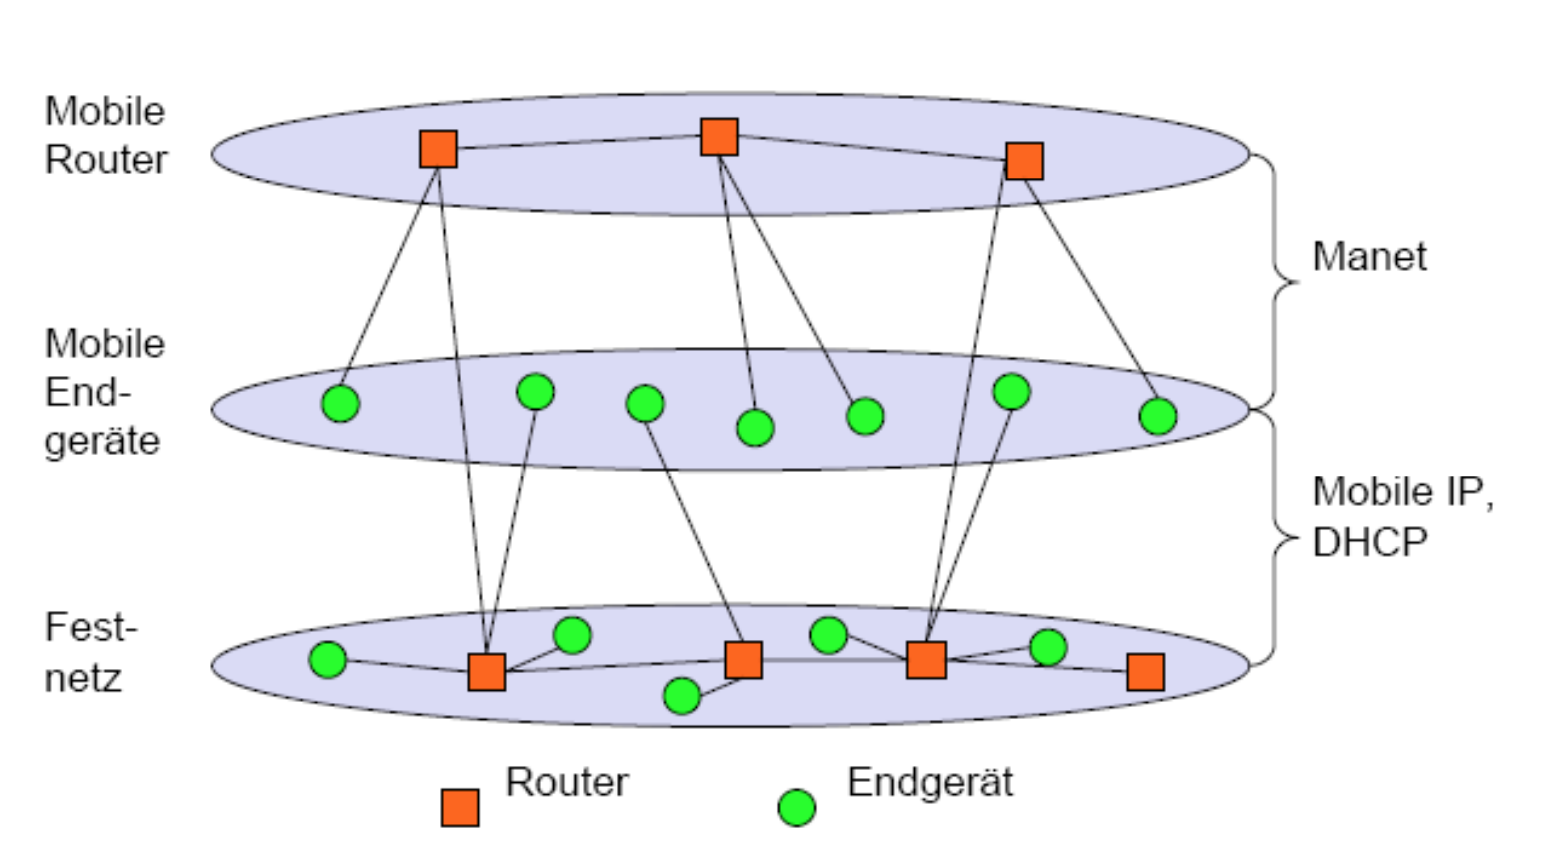
\includegraphics[scale=0.5]{Bilder/manet}
	\caption{Einordnung von MANETs\cite{d:timm}}
	\label{f:manet}
\end{figure}

MANETs zeichnen sich vor allem dadurch aus, dass sie keine feste Infrastruktur besitzen. Es herrscht innerhalb des Netzes eine dynamische Topologie, was bedeutet, dass zu jedem Zeitpunkt bestimmte Knoten wegfallen und neue dazukommen können. Dies führt dazu, dass bislang bekannte und zulässige Routen wegfallen, dafür aber auch neue Routen entstehen können. Unter den Geräten besteht eine spontane Vernetzung. Das bedeutet, dass jedes Gerät sowohl Endpunkt einer Übertragung sein kann, jedoch auch in der Lage sein muss, Daten weiterleiten zu können. Durch dieses Weiterleiten von Daten entsteht eine so genannte ‚Multihop-Umgebung‘, da die Daten nicht vom Sender direkt zum Empfänger gelangen, sondern den Empfänger über mehrere Zwischenstationen erreichen. \\

\begin{figure}[H] 
	\centering
	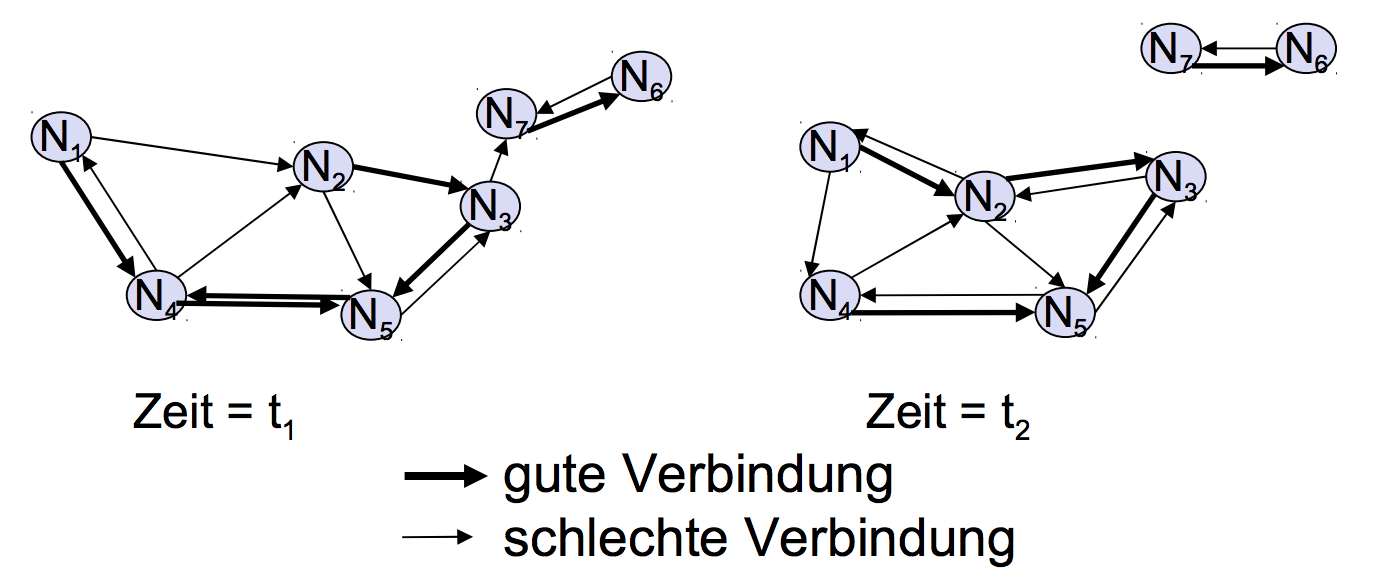
\includegraphics[scale=0.5]{Bilder/manetconnection}
	\caption{Mögliche Verbindungen eines Beispiel MANETs\cite{d:timm}}
	\label{f:manetconnection}
\end{figure}

Mobile Ad-hoc Netzwerke besitzen eine stark begrenzte Bandbreite. Da sie meistens auf stromsparende Übertragungsprotokolle setzen, können dementsprechend auch nur geringe Mengen an Daten übertragen werden. Des Weiteren bestehen zumeist durch die unterschiedlichen Übertragungsleistungen der Geräte asymmetrische Verbindungen, welche sich für die Übertragung von Daten innerhalb des Netzes besser eignen.\\

Ein Problem bei MANETs stellt die beschränkte Möglichkeit der Energieversorgung dar, da die Endgeräte meistens abhängig von Batterien oder Akkus sind. Durch die hohe Menge an Geräten in einem Netz steigt dazu die Summe des potenziellen Energiebedarfes pro Gerät weiter an. Auch die Sicherung des Netzes vor physischen Angriffen ist stark beschränkt. So sind z.B. Denial-of-Service-Attacken (DoS), Überwachungsangriffe oder auch das Verfälschen von Nachrichten oft leicht zu realisieren \cite{d:timm}.

\subsection{Routingprotokolle}\label{ss:Routingprotokolle}

Klassische Routingprotokolle versagen bei dem Versuch, sie innerhalb von mobilen Ad-hoc Netzwerken einzusetzen. Gründe dafür sind folgende: \\

MANETs zeichnen sich durch eine hohe Dynamik aus, das Netz verändert sich spontan, schnell und ständig. Klassische Protokolle besitzen eine zu langsame Konvergenz, um dem Anspruch der sich ständig verändernden Ad-hoc Netze gerecht zu werden und sind somit nicht geeignet.\\

Ad-hoc Netze besitzen wie bereits erwähnt meist eine geringe Bandbreite. Hinzu kommt, dass den angeschlossenen Knoten und Geräten nur eine gewisse Rechenleistung zur Verfügung steht. Sie sind somit mit klassischen Routingprotokollen überfordert, da diese meist viel Rechenleistung und Übertragungsleistung erfordern, welche mit den mobilen Geräten nicht realisierbar sind. Der Overhead der klassischen Protokolle ist also für diese Art von Netzwerken zu groß. \\

Es gibt in mobilen Ad-hoc Netzen gewisse Metriken, die beim Betrieb berücksichtigt werden müssen. Die klassischen Protokolle interessieren sich nicht für diese Metriken und lassen sie außen vor. Bei der Auswahl von Routen müssen unter anderem folgende Aspekte betrachtet werden:
\begin{itemize}
	\item Batterielaufzeit der Geräte
	\item Zeit der Verbindung zwischen zwei Geräten
	\item Energiebedarf
	\item Zuverlässigkeit der Verbindung
\end{itemize} 

Zusammengefasst lässt sich sagen, dass Routingprotokolle für MANETs vor allem eine große Skalierbarkeit im Hinsicht auf eine große Anzahl von Geräten, Flexibilität und Effizienz im Hinblick auf Komplexität, Energieverbrauch und Speicherverbrauch erfordern. Diese werden mittlerweile intensiv erforscht, da Ad-hoc Netze im Zusammenhang mit dem ‚Internet of Things‘ (IoT) oder auch dem ‚Internet Of Everything‘ (IoE) zunehmend an Bedeutung gewinnen \cite{d:timm}. \\

Im Folgenden sollen die Protokolle OLSR, AODV und CGSR kurz aufgezeigt und erklärt werden.

\subsubsection{OLSR}\label{ss:OLSR}

\subsubsection{AODV}\label{ss:AODV}

\subsubsection{CGSR}\label{ss:CGSR}

